\section{Bubbles}
\label{sec:bubbles}

The system is a square box of side $L$. The initial condition is a
circular domain with $\phi>0$ inside, of radius $R_0=L/6$, centred in
the box. The force $F$ is increased quasistatically, and the last pinned
configuration before the interface comes within three lattice sites of
the box boundary is retained. We call this the depinning configuration.
We use the closed outer contour, with area $A$ and area centroid
$\boldsymbol c$, and define $R=(A/\pi)^{1/2}$.

We also construct an area-preserving profile.
If a ray from $\boldsymbol c$ at angle $\theta$ intersects the dominant
contour at ordered radii $r_1<\cdots<r_{2m+1}$, its radius is
\begin{equation}
 h_\theta(\theta)=\Big[\sum_{j=1}^{2m+1}(-1)^{j+1}r_j(\theta)^2\Big]^{1/2},
 \qquad \theta\in[0,2\pi).
 \label{eq:area-radius}
\end{equation}
This is the radius of the occupied area in that direction, so that
$\frac12\int_0^{2\pi}h_\theta^2\,d\theta=A$.
Detached islands and hole boundaries are omitted.
We sample $\lceil2\pi R\rceil$ rays, about one per lattice spacing at
radius $R$, and use $u=R\theta$ with period $T=2\pi R$ in
Eq.~\eqref{eq:height-modes}.

We also measure a local width that does not refer to $\boldsymbol c$.
The contour is resampled at uniform arc length, with spacing at most one
lattice spacing, and divided into arcs of length $\ell$ whose starting
points are separated by $\ell/4$.
Each arc is compared with a reference curve, and $d_i$ denotes the
deviation of its $i$th point from it.
We use two references.
The first is the straight line through the mean point of the arc,
oriented along the mean unit tangent, that is, along the chord joining
the two ends of the arc. Then $d_i$ is the distance from this line and
$X$ is the chord length.
The second is a cubic, with $x(s)$ and $y(s)$ fitted separately by least
squares over the arc. Then $d_i$ is measured along the normal of the
cubic and $X$ is its length.
The local width is
\begin{equation}
 w^2(\ell)=\Big\langle\frac1n\sum_{i=1}^{n}d_i^2\Big\rangle,
 \label{eq:arc-width}
\end{equation}
where $n$ is the number of points of an arc and the average runs over
the arcs of each contour and then over contours, with equal weight per
contour. We use $\ell\leq P_{\min}/4$, and plot $w$ against the mean of
$X$ at the same $\ell$.
The line removes the mean position and the orientation of an arc, and
the cubic also removes its curvature, so that $w\propto X^\zeta$ for a
self-affine interface with $\zeta<2$ and $\zeta<4$, respectively.
The local exponent is $d\ln w/d\ln X$, with $95\%$ bootstrap intervals
over contours.

\subsection{Isotropic disorder}
\label{sec:bubble-isotropic}

For $a=0$ we analyse $128,64,32,16$ realizations at
$L=1024,2048,4096,8192$, respectively.
Figure~\ref{fig:bubble-profiles} shows the contour, $h_\theta(\theta)$
and $h_s(s)$ for the same realization.

\begin{figure}[H]
 \centering
 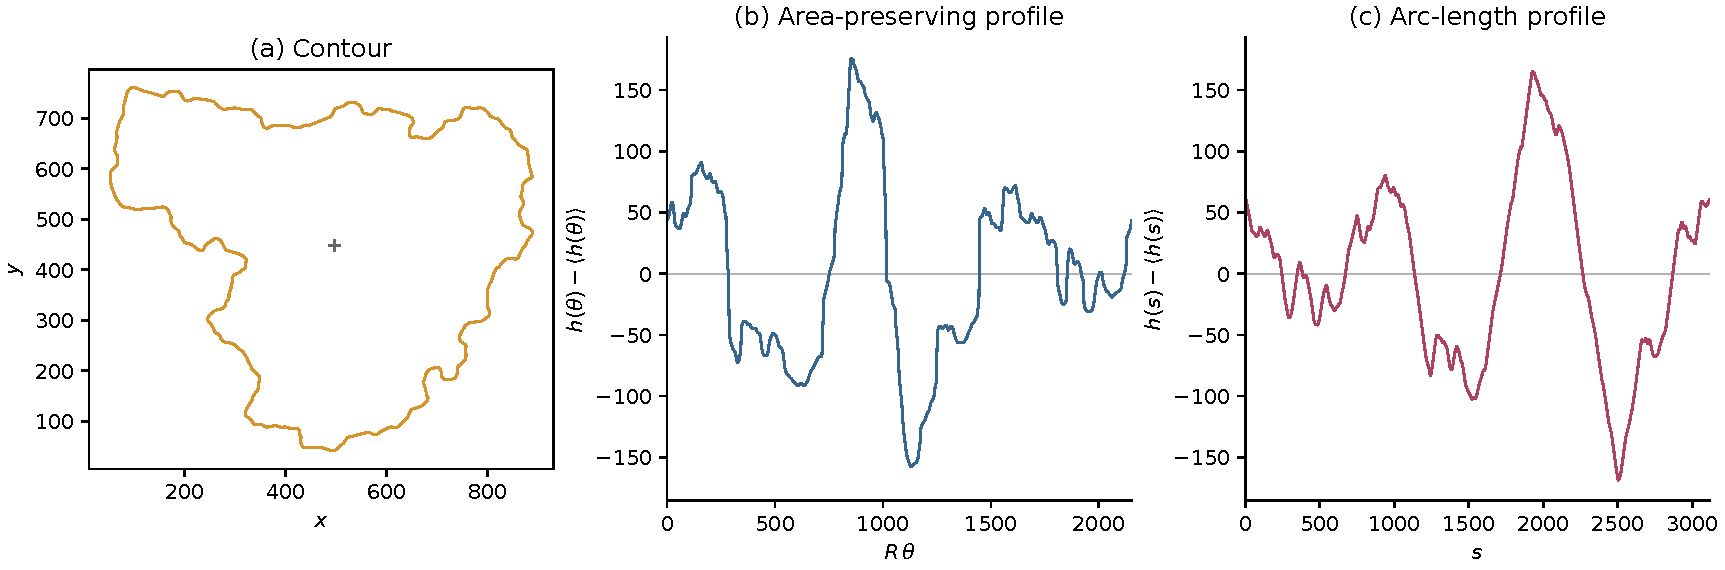
\includegraphics[width=\linewidth]{fig7_bubble_profiles.pdf}
 \caption{Bubble with isotropic disorder at $L=1024$,
 with contour length $P=3118.33$ and $R=342.67$.
 (a) Full depinning contour; the cross marks the area centroid.
 (b) Area-preserving profile $h(\theta)$, defined from the alternating
 sum of the squared crossing radii on each ray, versus $R\theta$.
 (c) Height $h(s)=|\boldsymbol r(s)-\boldsymbol c|$ along the contour,
 parametrized by arc length $s\in[0,P)$.
 In (b,c), the means $\langle h(\theta)\rangle$ and
 $\langle h(s)\rangle$ are subtracted, respectively.}
 \label{fig:bubble-profiles}
\end{figure}

The mean perimeter grows approximately as
$\mathbb E[P]\propto L^{1.21}$.
Figure~\ref{fig:bubble-scaling}(a) compares this growth with $L$
and $L^{1.25}$.
Figures~\ref{fig:bubble-scaling}(b,c) show $S(n)$ for $h_\theta$ and
$h_s$, with lines of slope $-3.5$ (qEW) and $-2.26$ (qKPZ).
At $L=8192$ the arc-length spectrum gives $\zeta\simeq0.92$ for the
first quarter of the modes, $2\leq n\leq45$, and $1.07$ at larger $n$;
at $q\leq0.03$ the fitted exponent is $\zeta_s\simeq1.00$.
The $h_\theta$ spectra are flatter, with $\zeta\simeq0.77$ and $0.93$,
as $h_x$ is for flat interfaces.
Neither representation follows the qKPZ slope.

\begin{figure}[H]
 \centering
 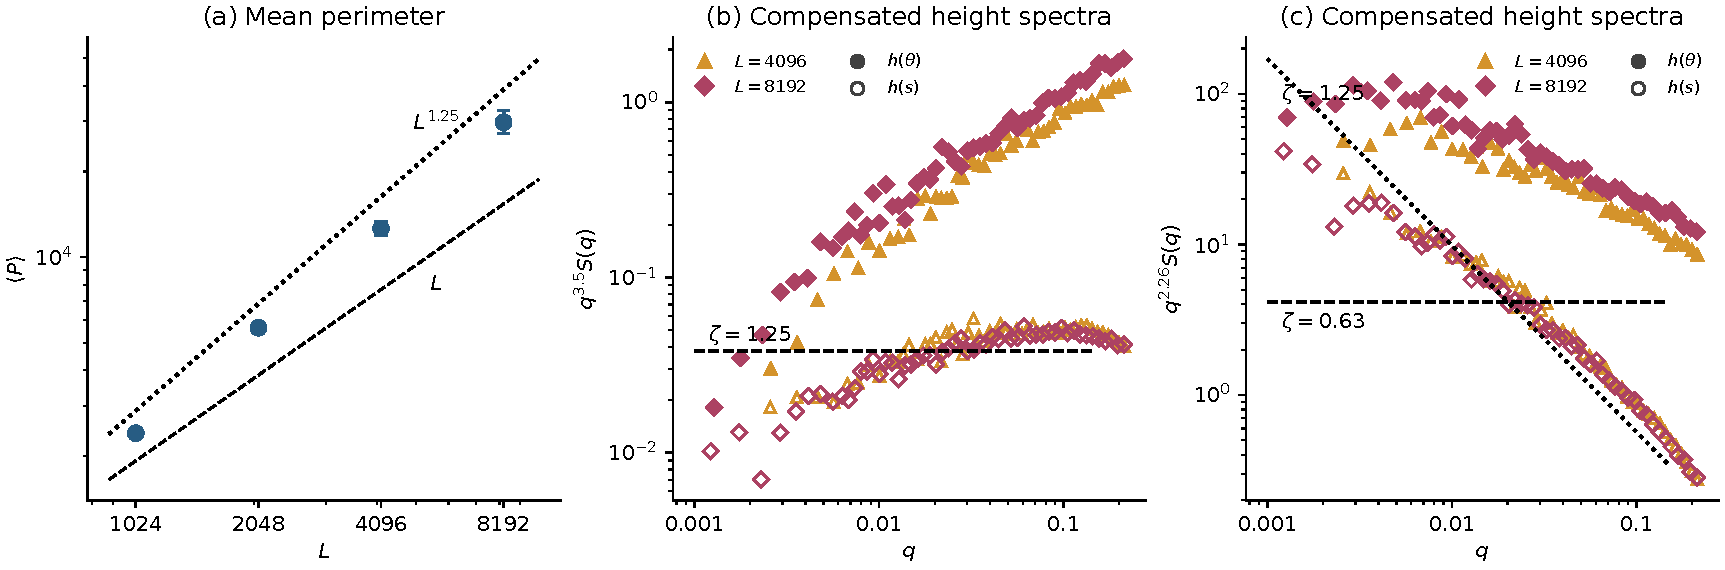
\includegraphics[width=\linewidth]{fig8_bubble_scaling.pdf}
 \caption{Bubbles with isotropic disorder and $R_0=L/6$.
 (a) Mean perimeter versus $L$.
 Error bars give $95\%$ bootstrap intervals for the mean.
 The black dashed and dotted lines have slopes $1$ and $1.25$, respectively.
 (b) Spectra $S(n)=\langle|\widehat h_n|^2\rangle$ of $h_\theta(\theta)$
 versus the mode index $n$ for $L=4096$ and $8192$, with
 $2\leq n\leq45L/2048$.
 (c) The same for $h_s(s)$.
 In (b,c), the black dashed and dotted lines have slopes $-3.5$
 ($\zeta=1.25$) and $-2.26$ ($\zeta=0.63$), with freely chosen
 amplitudes.
 Each contour has equal weight in the disorder average.}
 \label{fig:bubble-scaling}
\end{figure}

Figures~\ref{fig:bubble-arc-line} and~\ref{fig:bubble-arc-cubic} show
the local width, Eq.~\eqref{eq:arc-width}, for the line and the cubic.
For flat isotropic interfaces at $L_x=2048$, analysed in the same way,
the arcs are taken along the periodic contour.
For both references $w(X)$ does not depend on $L$ and coincides with that
of the flat interfaces.
With the line, the local exponent decreases from $1.25$ at $X\simeq90$
to $1.17$ at $X\simeq360$ for $L=8192$.
With the cubic, it decreases from $1.25$ at $X\simeq190$ to $1.18$ at
$X\simeq440$.
For $X\lesssim100$ the local exponent depends on the reference and
exceeds $1.25$.
No range is consistent with $\zeta=0.63$.
The derivative with respect to $\ln\ell$ instead of $\ln X$ is smaller
and falls below $1$ at large $\ell$, because $X/\ell$ decreases with
$\ell$.

\begin{figure}[H]
 \centering
 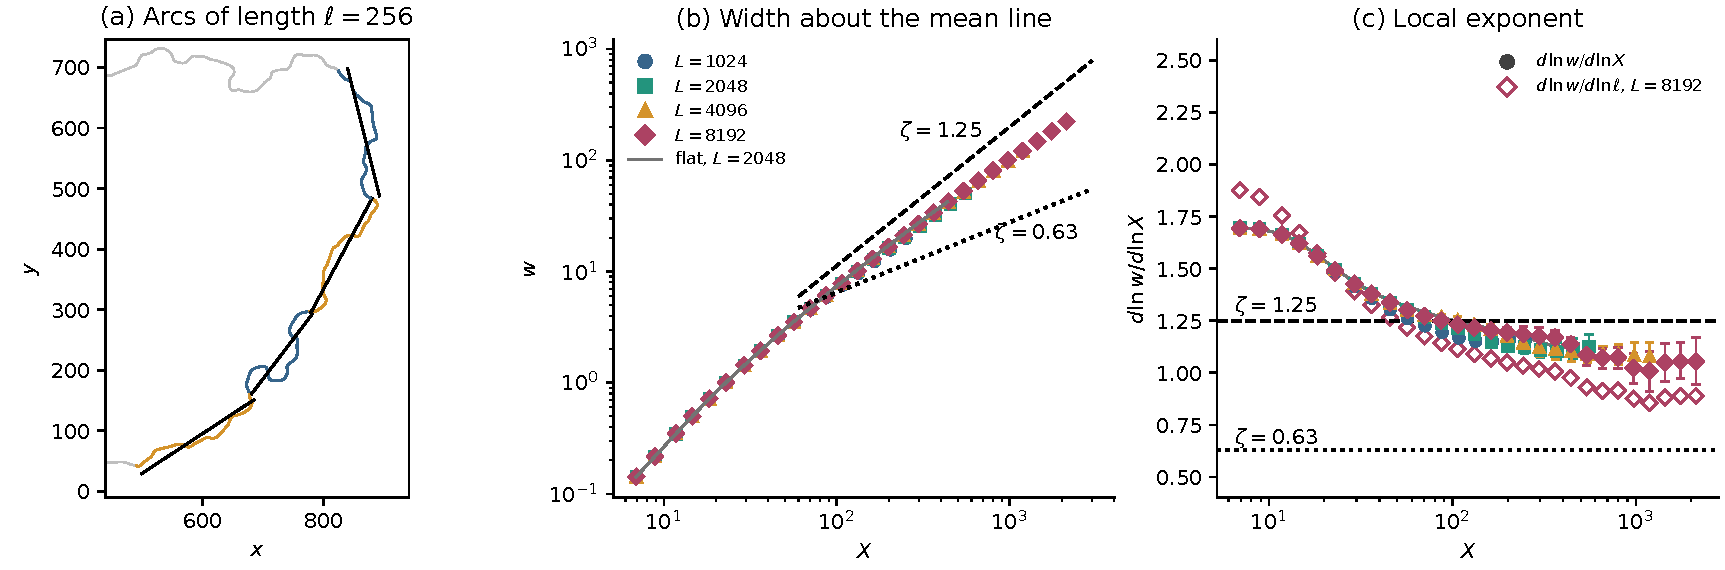
\includegraphics[width=\linewidth]{fig11_bubble_arc_width_line.pdf}
 \caption{Local width of bubbles with isotropic disorder about the mean
 line of arcs of length $\ell$.
 (a) Four consecutive arcs with $\ell=256$ of the contour of
 Fig.~\ref{fig:bubble-profiles}, and their mean lines (black).
 (b) Width $w$ versus the chord length $X$.
 The grey line gives flat isotropic interfaces at $L_x=2048$.
 The dashed and dotted lines have slopes $1.25$ and $0.63$, respectively,
 with freely chosen amplitudes.
 (c) Local exponent $d\ln w/d\ln X$, with $95\%$ bootstrap intervals.
 Open symbols give $d\ln w/d\ln\ell$ for $L=8192$.}
 \label{fig:bubble-arc-line}
\end{figure}

\begin{figure}[H]
 \centering
 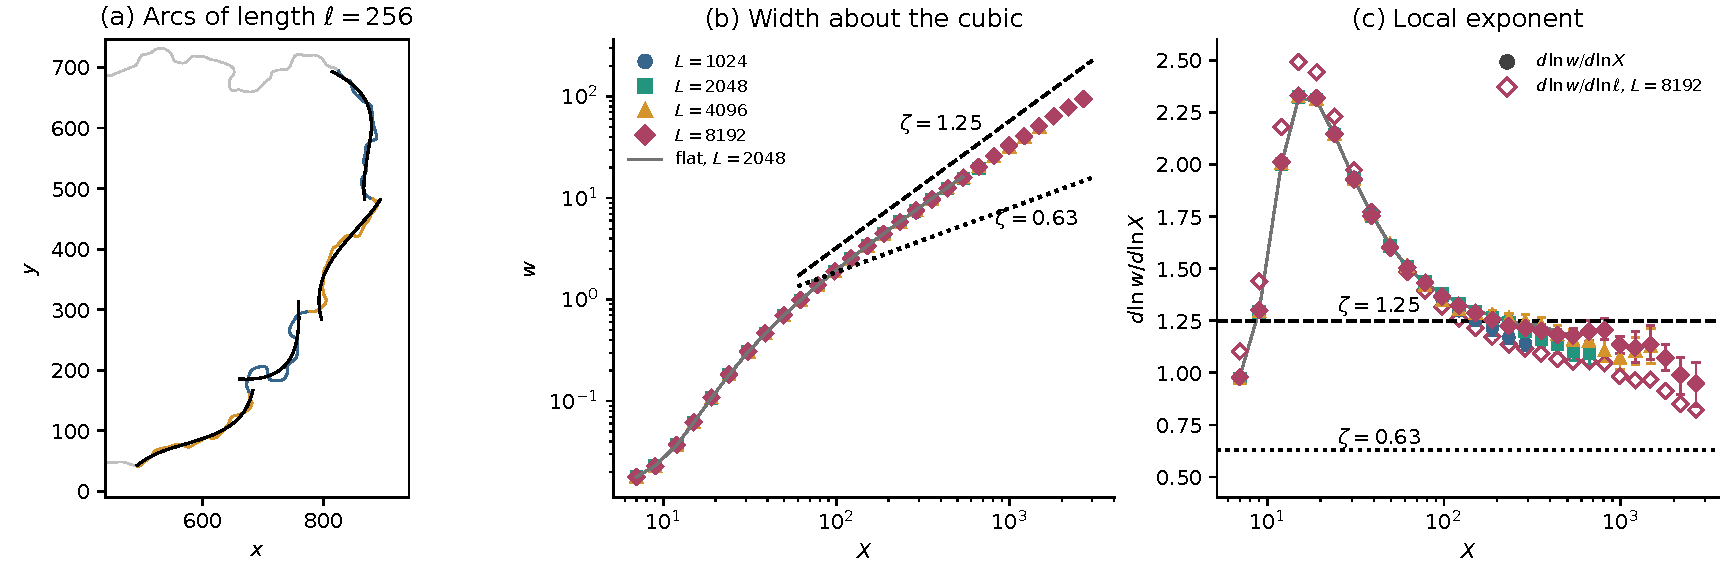
\includegraphics[width=\linewidth]{fig12_bubble_arc_width_cubic.pdf}
 \caption{As Fig.~\ref{fig:bubble-arc-line}, with a cubic fitted to each
 arc as the reference. $X$ is the length of the cubic.}
 \label{fig:bubble-arc-cubic}
\end{figure}

\subsection{Anisotropic disorder}
\label{sec:bubble-anisotropic}

For $a=1$ we use $\beta=0$, so $\hat{\boldsymbol b}$ is along the $x$
axis, and the same system sizes and numbers of realizations as for
$a=0$. A bubble contour contains every orientation:
it is edge-like where its normal is parallel to $\hat{\boldsymbol b}$
and screw-like where its normal is perpendicular to it.
Figure~\ref{fig:bubble-aniso-profiles} shows a depinning configuration
elongated perpendicular to $\hat{\boldsymbol b}$.
For $L\geq2048$ the median depinning configuration extends over
$0.86$--$0.89$ of the box height, so the extent of the screw-like
tips is set by the box boundary.

\begin{figure}[H]
 \centering
 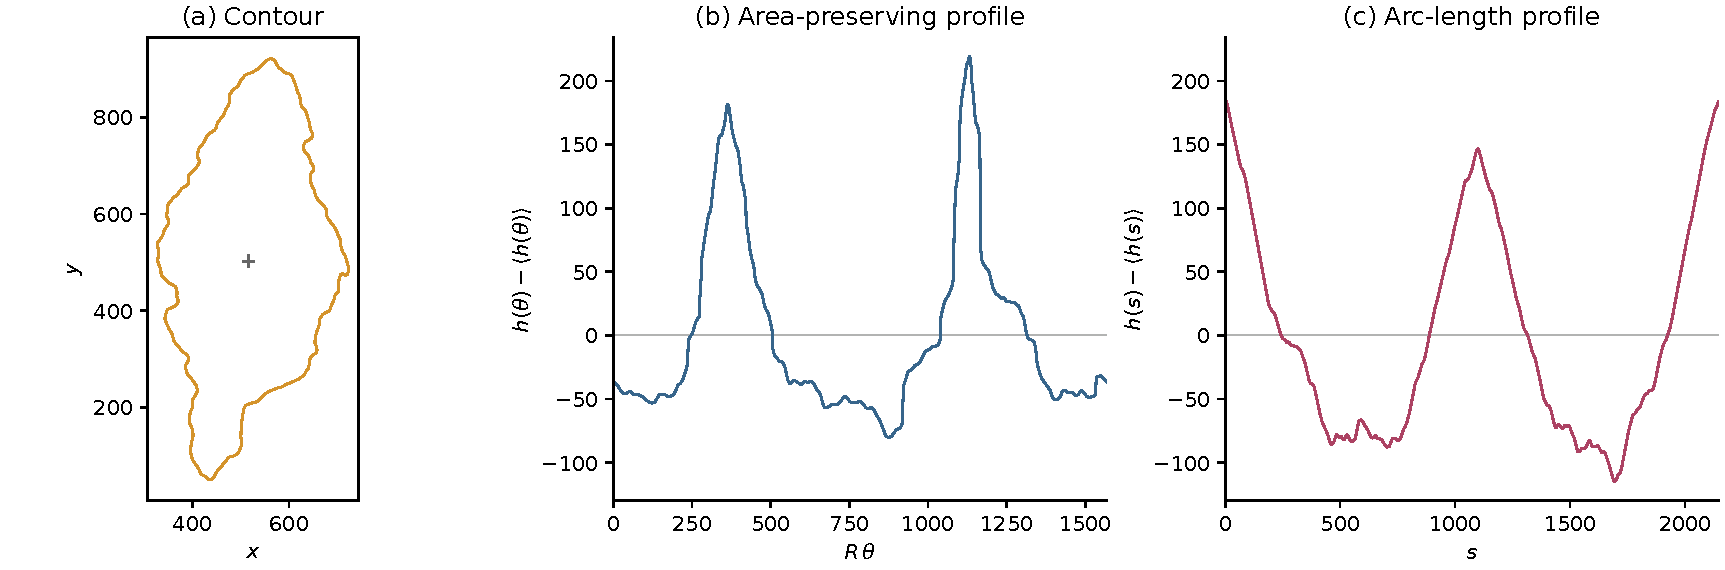
\includegraphics[width=\linewidth]{fig9_bubble_anisotropic_profiles.pdf}
 \caption{Bubble with anisotropic disorder ($a=1$, $\beta=0$) at
 $L=1024$, with perimeter $P=2146.47$ and $R=249.66$.
 (a) Full depinning contour; the cross marks the area centroid.
 (b) Area-preserving profile $h(\theta)$ versus $R\theta$.
 (c) Height $h(s)=|\boldsymbol r(s)-\boldsymbol c|$ along the contour,
 parametrized by arc length $s\in[0,P)$.
 In (b,c), the means $\langle h(\theta)\rangle$ and
 $\langle h(s)\rangle$ are subtracted, respectively.}
 \label{fig:bubble-aniso-profiles}
\end{figure}

The mean perimeter grows approximately as
$\mathbb E[P]\propto L^{1.20}$, as shown in
Fig.~\ref{fig:bubble-aniso-scaling}(a).
The ratio $\mathbb E[P]/L$ increases from $2.04$ at $L=1024$
to $3.11$ at $L=8192$.
Figures~\ref{fig:bubble-aniso-scaling}(b,c) show $S(n)$ for $h_\theta$
and $h_s$.
The arc-length spectra follow the $\zeta=1.25$ line over all the modes
shown, with $\zeta\simeq1.24$ at $L=8192$; at $q\leq0.03$ the fitted
exponent is $\zeta_s\simeq1.33$.
The $h_\theta$ spectra are dominated at small $n$ by the elongation of
the contour, which enhances the even modes $n=2,4$.
No representation follows the qKPZ slope.

\begin{figure}[H]
 \centering
 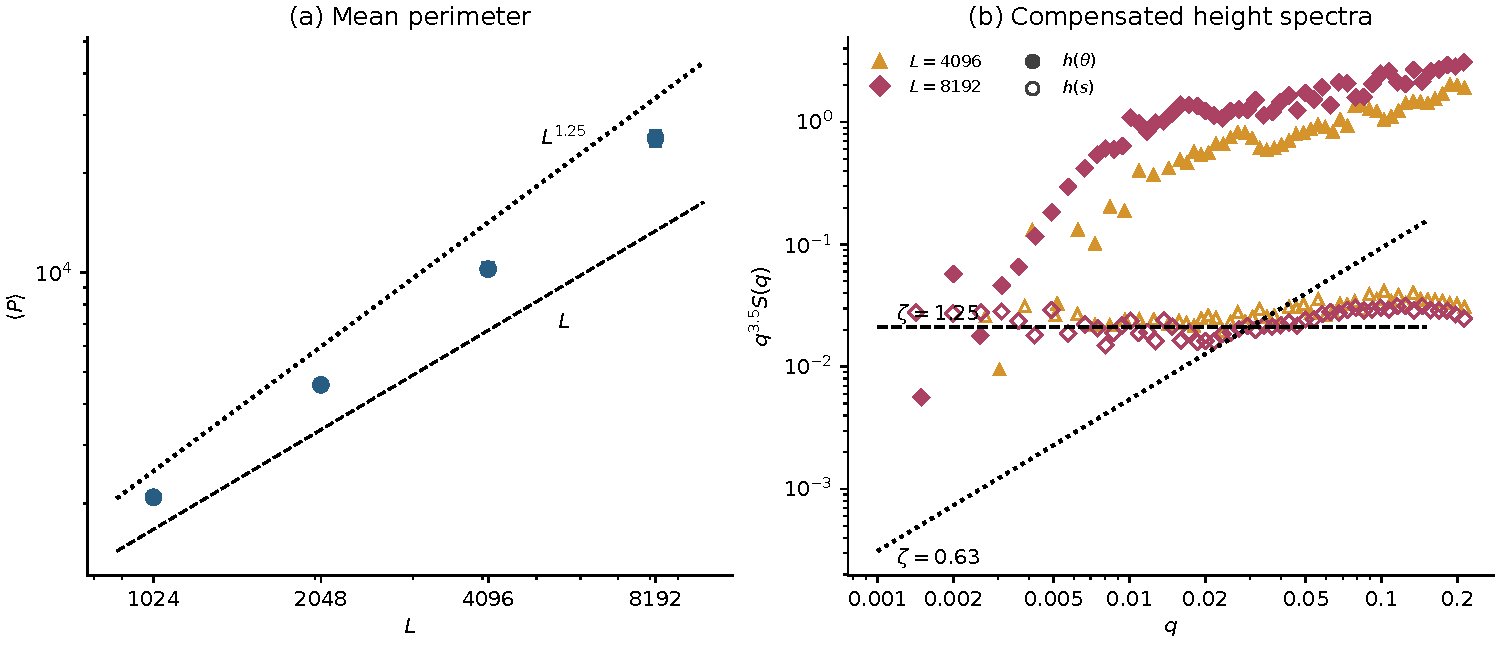
\includegraphics[width=\linewidth]{fig10_bubble_anisotropic_scaling.pdf}
 \caption{Bubbles with anisotropic disorder ($a=1$, $\beta=0$) and
 $R_0=L/6$.
 (a) Mean perimeter versus $L$.
 Error bars give $95\%$ bootstrap intervals for the mean.
 The black dashed and dotted lines have slopes $1$ and $1.25$,
 respectively.
 (b) Spectra $S(n)=\langle|\widehat h_n|^2\rangle$ of $h_\theta(\theta)$
 versus the mode index $n$ for $L=4096$ and $8192$, with
 $2\leq n\leq45L/2048$.
 (c) The same for $h_s(s)$.
 In (b,c), the black dashed and dotted lines have slopes $-3.5$
 ($\zeta=1.25$) and $-2.26$ ($\zeta=0.63$), with freely chosen
 amplitudes.
 Each contour has equal weight in the disorder average.}
 \label{fig:bubble-aniso-scaling}
\end{figure}

For the local width, each arc is classified by the direction of the
normal to its chord, folded into $[0^\circ,90^\circ]$ from
$\hat{\boldsymbol b}$. Arcs whose normal is within $30^\circ$ of
$\hat{\boldsymbol b}$ are edge-like, arcs whose normal is within
$30^\circ$ of the perpendicular direction are screw-like, and the others
are not used. A contour enters the average at a given $\ell$ if it has
arcs of that class, and $\ell$ is retained if at least $80\%$ of the
contours enter. For comparison, flat edge ($\beta=90^\circ$) and screw
($\beta=0^\circ$) interfaces with $a=1$ and $L_x=2048$ are analysed with
all their arcs.
Figures~\ref{fig:bubble-aniso-arc-line}
and~\ref{fig:bubble-aniso-arc-cubic} show the results.

For edge-like arcs, $w(X)$ coincides with that of flat edge interfaces
up to $X\simeq200$ for both references.
With the line, the local exponent at $L=8192$ decreases to $0.81$ for
$230\lesssim X\lesssim360$ and then increases, reaching $1$ at
$X\simeq850$.
For flat edge interfaces it continues to decrease, to $0.69$--$0.70$
for $360\lesssim X\lesssim460$.
With the cubic, the minimum is $0.86$--$0.87$ at $X\simeq470$--$580$
for edge-like arcs, and $0.78$ at $X\simeq470$ for flat edge interfaces.

Screw-like arcs are strongly folded: with the line, $X/\ell=0.37$ at
$\ell=645$, and at $X\simeq240$ the width is about seven times that of
edge-like arcs. The local exponent is between $1.3$ and $1.8$, with
wide intervals. For flat screw interfaces it increases from $1.06$ at
$X\simeq140$ to about $2$ at $X\simeq1000$, so that the line does not
remove their large-scale bending.
With the cubic, $w$ for screw-like arcs is about $1.3$ times that of
edge-like arcs, and the local exponent is $1.07$--$1.18$ for
$150\lesssim X\lesssim800$; flat screw interfaces give $0.97$--$1.0$ for
$370\lesssim X\lesssim580$.

\begin{figure}[H]
 \centering
 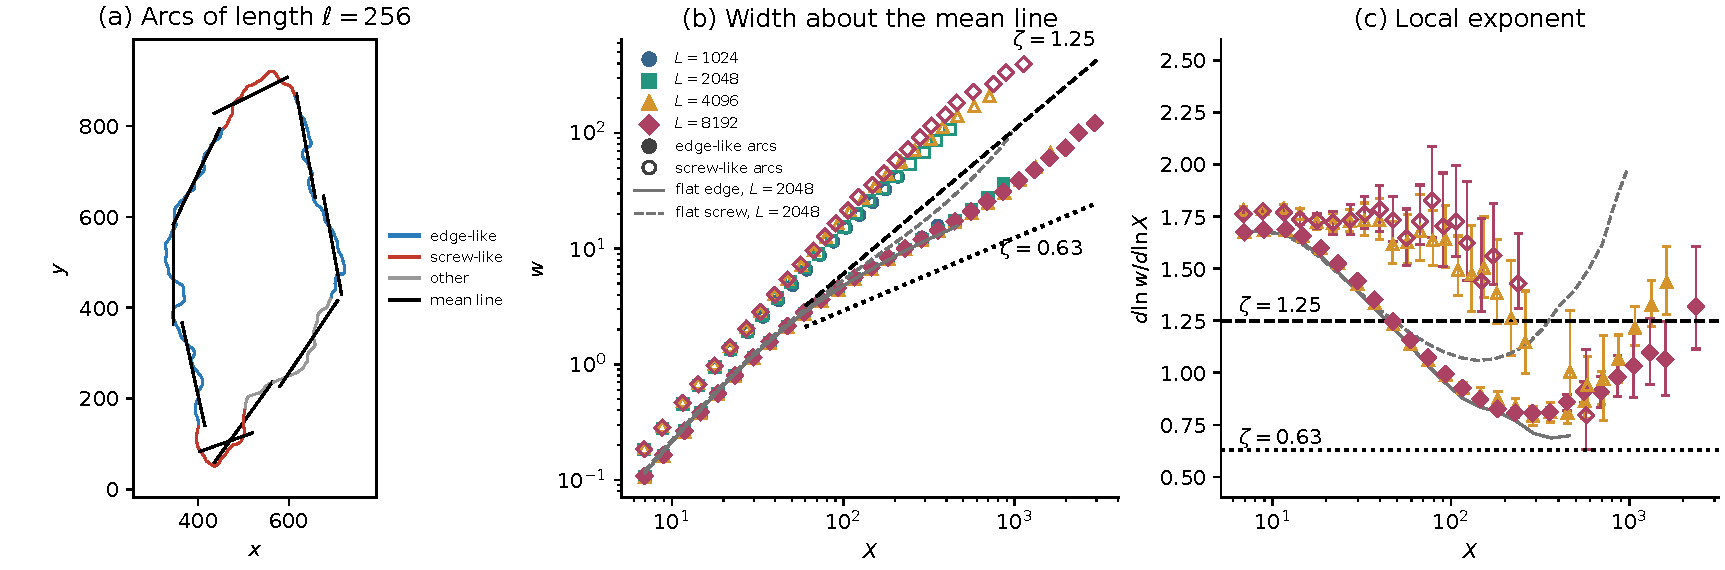
\includegraphics[width=\linewidth]{fig13_bubble_anisotropic_arc_width_line.pdf}
 \caption{Local width of bubbles with anisotropic disorder ($a=1$,
 $\beta=0$) about the mean line of arcs of length $\ell$.
 (a) Consecutive arcs with $\ell=256$ of the contour of
 Fig.~\ref{fig:bubble-aniso-profiles}, coloured by class, and their mean
 lines (black).
 (b) Width $w$ versus the chord length $X$.
 Filled and open symbols represent edge-like and screw-like arcs,
 respectively. The solid and dashed grey lines give flat edge and screw
 interfaces at $L_x=2048$.
 The black dashed and dotted lines have slopes $1.25$ and $0.63$,
 with freely chosen amplitudes.
 (c) Local exponent $d\ln w/d\ln X$ for $L=4096$ and $8192$, with $95\%$
 bootstrap intervals; points with intervals wider than $0.5$ are omitted.}
 \label{fig:bubble-aniso-arc-line}
\end{figure}

\begin{figure}[H]
 \centering
 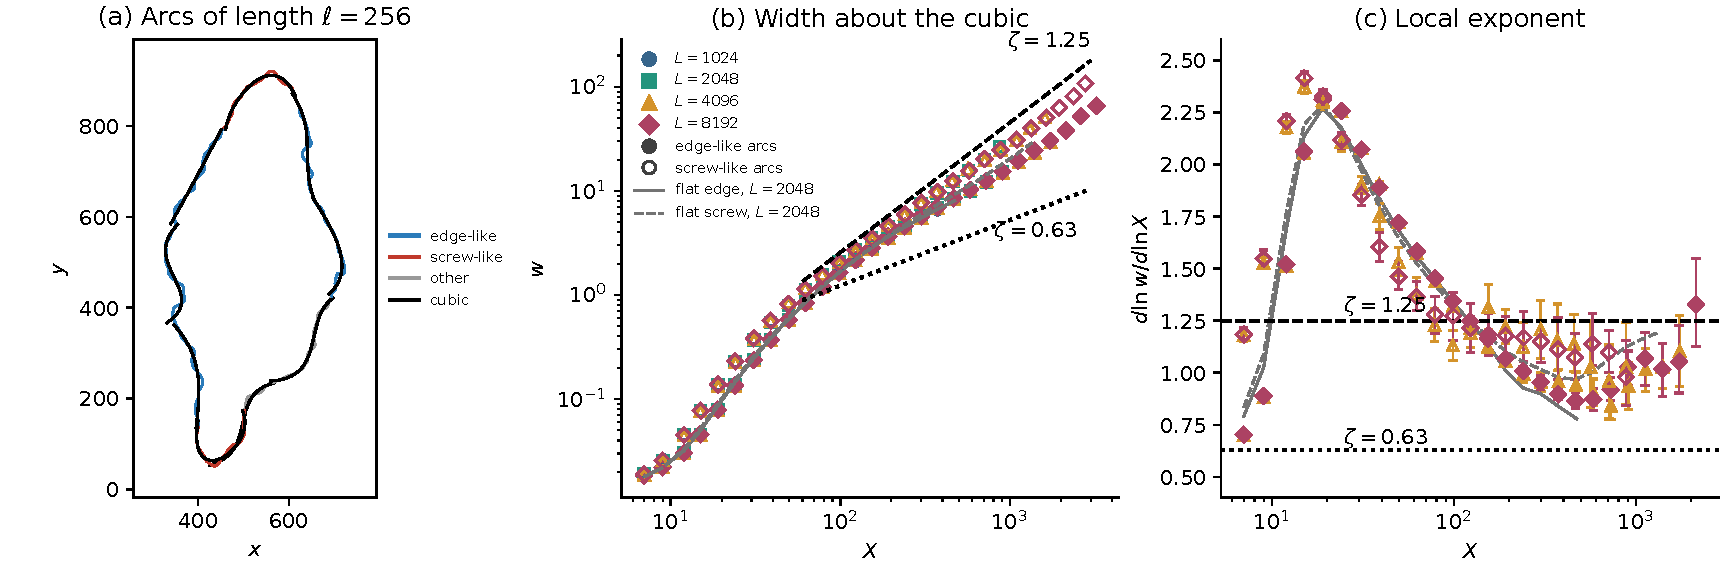
\includegraphics[width=\linewidth]{fig14_bubble_anisotropic_arc_width_cubic.pdf}
 \caption{As Fig.~\ref{fig:bubble-aniso-arc-line}, with a cubic fitted to
 each arc as the reference. $X$ is the length of the cubic.}
 \label{fig:bubble-aniso-arc-cubic}
\end{figure}
